\documentclass[runningheads]{llncs}

\usepackage{amssymb}
\usepackage{amsmath}
%% The amsthm package provides extended theorem environments

% \usepackage{amsthm}
% AM commented out because it clashes with proof, etc

%% The lineno packages adds line numbers. Start line numbering with
%% \begin{linenumbers}, end it with \end{linenumbers}. Or switch it on
%% for the whole article with \linenumbers.
\usepackage{lineno}

%% Use package enumitem to align enumeration and itemization
\usepackage{enumitem}
\usepackage{listings}
\usepackage{courier}           % for the courier font (optional)
\usepackage{multicol}          % for two equations side by side
\usepackage[justification=centering]{caption}
\usepackage{xcolor}
\usepackage{stmaryrd}
\usepackage{hyperref}
%\usepackage{cleveref}
\usepackage{hieroglf}
\usepackage{scalerel}
\usepackage{tikz}
\usepackage{pgfplots}


\hypersetup{ % play with these to change the look of hyperlinks
    colorlinks=true,
    linkcolor=black,
    filecolor=magenta,
    urlcolor=blue,
    citecolor=black
}

\newcommand{\coq}{\scalebox{.6}{\textpmhg{\Ha}}}

% required by LNCS
\renewcommand\UrlFont{\color{blue}\rmfamily}

\colorlet{red}{red!80!black}
\colorlet{green}{green!50!black}

%% NEW COMMANDS =============================================

\lstdefinestyle{myStyle}{
%	language=Coq,
    keywords={Inductive,Require,Import,Definition,Fixpoint,match,with,end,let,in,fix},
	basicstyle=\normalfont\footnotesize\tt,
    keywordstyle=\color{green}, % Blue clashes with the cyan links. Change if you want.
	stepnumber=1,
	tabsize=2,
    numbers=none,
    numberstyle=\tiny,
    numbersep=5pt,
	showspaces=false,
    escapechar=`,
	showstringspaces=false
}
%basicstyle=\fontsize{10}{11}\selectfont\ttfamily,

\lstdefinestyle{myTinyStyle}{
%   language=Coq,
    keywords={Inductive,Require,Import,Definition,Fixpoint,match,with,end,let,in,fix},
    basicstyle=\normalfont\fontsize{8.2}{8.5}\tt,
    keywordstyle=\color{green}, % Blue clashes with the cyan links. Change if you want.
    stepnumber=1,
    tabsize=2,
    numbers=none,
    numberstyle=\tiny,
    numbersep=5pt,
    showspaces=false,
    escapechar=`,
    showstringspaces=false
}

\lstset{style=myStyle}
\makeatletter
\newlength{\@mli}
\newcommand{\mli}[1]{%
  \settowidth{\@mli}{\lstinline/#1/}
  \hspace{-.5ex}\begin{minipage}[t]{\@mli}\lstinline/#1/\end{minipage}}
\makeatother
\newcommand{\li}[1]{\ifmmode\mbox{\mli{#1}}\else\mbox{\lstinline/#1/}\fi}

\newcommand\hide[1]{}

\newenvironment{centermath}
 {\begin{center}$\displaystyle}
 {$\end{center}}

\renewcommand{\note}[2][polish]{{\color{red} #2}{\marginpar{\tiny \color{blue} #1}}}
\renewcommand{\implies}{\Rightarrow}
\renewcommand{\iff}{\Leftrightarrow}

\title{A Machine-Checked C Implementation of Dijkstra's Shortest Path Algorithm}
\subtitle{Short Paper}
\titlerunning{Machine-Checked Dijkstra}
%optional, please use if title is longer than one line

\begin{document}

\author{Anshuman Mohan \and Aquinas Hobor}
\authorrunning{A. Mohan, A. Hobor}

%\author{Linh Tran \and Anshuman Mohan \and Aquinas Hobor}
%\authorrunning{L. Tran, A. Mohan, A. Hobor}
% First names are abbreviated in the running head.
% If there are more than two authors, 'et al.' is used.
%
\institute{National University of Singapore \\
\email{\{mohan,hobor\}@comp.nus.edu.sg}}


\maketitle
%\begin{frontmatter}

%% Title, authors and addresses

%% use the tnoteref command within \title for footnotes;
%% use the tnotetext command for theassociated footnote;
%% use the fnref command within \author or \address for footnotes;
%% use the fntext command for theassociated footnote;
%% use the corref command within \author for corresponding author footnotes;
%% use the cortext command for theassociated footnote;
%% use the ead command for the email address,
%% and the form \ead[url] for the home page:

%% \tnotetext[label1]{}
%% \author{Name\corref{cor1}\fnref{label2}}
%% \ead{email address}
%% \ead[url]{home page}
%% \fntext[label2]{}
%% \cortext[cor1]{}
%% \address{Address\fnref{label3}}
%% \fntext[label3]{}

%% use optional labels to link authors explicitly to addresses:
%% \author[label1,label2]{}
%% \address[label1]{}
%% \address[label2]{}

%\author{}

%\address{}


\begin{abstract}
\vspace{-2em}
We report on a machine-checked proof of correctness for 
Dijkstra’s one-to-all shortest path algorithm. 
Unlike previous work, we use classic textbook code written in C.
Our C code is executable and realistic but also has 
real-world complications. 
We prove full functional correctness, and not just program safety.
We show that Dijkstra’s algorithm suffers from potential overflow issues. 
The precise bound is nontrivial: we show that the intuitive guess 
fails, and provide a workable refinement.

\keywords{Dijkstra \and verification \and Coq}
\end{abstract}

%\end{frontmatter}

%% \linenumbers

%% main text

% \section{Overview}
% \label{sec: overview}
% 
Figure~\ref{fig:decorated} shows the code and proof
sketch of Dijkstra's algorithm. 
The code is implemented exactly as suggested 
by~\cite{clrs}, and so we elide a discussion 
of the algorithm itself. The heart of the formal verification is in the 
while loop's invariant, which is stated on line~\ref{code:whileinv}
and explained further in Figure~\ref{fig:defns}.
The source vertex $\m{src}$ is taken as a parameter. 
A destination vertex $\m{dst}$ falls into one of three
categories, and subsequently obeys one of three invariants:
\begin{enumerate}
\item $\m{inv\_popped}$: $\m{dst}$ has been fully processed, and has been
popped from the priority queue. 
A globally optimal path from $\m{src}$ 
to $\m{dst}$ exists, the cost of this path is logged in 
the \texttt{dist} array, and all the vertices visited by the path are also popped.
Further, the links of this path are correctly logged in the \texttt{prev} array.
\item $\m{inv\_unpopped}$: $\m{dst}$ is reachable in 
one hop from a ``\emph{mom}'' vertex, which is itself popped. 
This route is locally optimal: we cannot 
improve the cost by going via a \emph{different} popped vertex.
The \texttt{prev} array logs
\emph{mom} as the best-known way to reach $\m{dst}$, and the \texttt{dist}
array logs the cost of the path via \emph{mom} as the best-known cost.
\item $\m{inv\_unseen}$: no path is currently known from $\m{src}$ to $\m{dst}$.
\end{enumerate}

This three-part invariant is trivially true before the while loop. 
On line~\ref{code:pop}, the minimal vertex from the priority queue is popped, 
thus breaking the invariant.

First, we must show that the minimal vertex $\m{u}$ 
obeys $\m{inv\_popped}$. \emph{i.e.}, show that the locally 
optimal path to $\m{u}$ is, in fact, globally optimal. 
This comes from blah blah blah

\newcommand{\s}{11}
\begin{figure}[htbp]
  \centering
  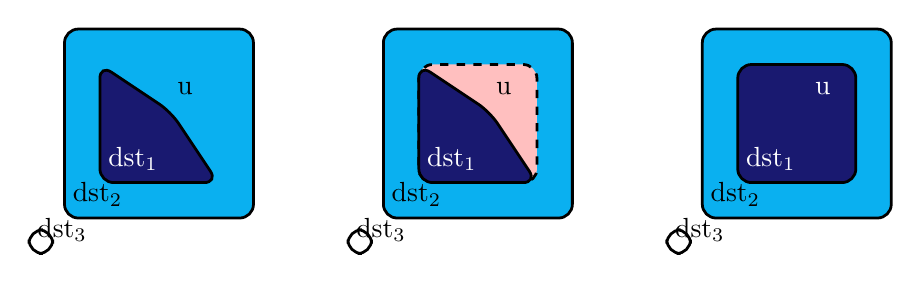
\begin{tikzpicture}[x=0.3cm, y=0.3cm,
      popped/.style={rounded corners=5pt, line width=1pt, draw, fill=MidnightBlue},
      fringe/.style={rounded corners=5pt, line width=1pt, draw, fill=ProcessBlue},
      popping/.style={rounded corners=5pt, line width=1pt, draw, dashed, fill=pink},
      unseen/.style={rounded corners=5pt, line width=1pt, draw}]
    \draw[unseen] (0,0) -- (\s,0) -- (\s,\s) -- (0,\s) -- cycle;
    \draw[fringe] (1.5,1.5) -- (9.5,1.5) -- (9.5,9.5) -- (1.5,9.5) -- cycle;
    \draw[popped] (3,3) -- (8,3) -- (6,6) -- (3,8) -- cycle;
    \node at (1.4,1) {dst$_3$};   
    \node at (2.9,2.5) {dst$_2$};   
    \node at (4.4,4) {\color{white}dst$_1$}; 
    \node at (6.6,7) {u};
    \tikzset{shift={(13.5,0)}}

    \draw[unseen] (0,0) -- (\s,0) -- (\s,\s) -- (0,\s) -- cycle;
    \draw[fringe] (1.5,1.5) -- (9.5,1.5) -- (9.5,9.5) -- (1.5,9.5) -- cycle;
    \draw[popping] (3,3) -- (8,3) -- (8,8) -- (3,8) -- cycle;
    \draw[popped] (3,3) -- (8,3) -- (6,6) -- (3,8) -- cycle;
    \node at (1.4,1) {dst$_3$};   
    \node at (2.9,2.5) {dst$_2$};   
    \node at (4.4,4) {\color{white}dst$_1$}; 
    \node at (6.6,7) {u};     

    \tikzset{shift={(13.5,0)}}

    \draw[unseen] (0,0) -- (\s,0) -- (\s,\s) -- (0,\s) -- cycle;
    \draw[fringe] (1.5,1.5) -- (9.5,1.5) -- (9.5,9.5) -- (1.5,9.5) -- cycle;
    \draw[popped] (3,3) -- (8,3) -- (8,8) -- (3,8) -- cycle;
    \node at (1.4,1) {dst$_3$};   
    \node at (2.9,2.5) {dst$_2$};   
    \node at (4.4,4) {\color{white}dst$_1$}; 
    \node at (6.6,7) {\color{white}u};       
  \end{tikzpicture}
  \caption{Popping $\m{u}$}  
\end{figure}

Next, we must account for the ripple effect that popping 
$\m{u}$ could have had on the other vertices. 
In particular, it is possible that a vertex obeying $\m{inv\_unpopped}$ can
improve its cost via $\m{u}$, and that an unreachable vertex 
obeying $\m{inv\_unseen}$ can now be reached via $\m{u}$. 
The for loop repairs these breakages by 
checking if a path via $\m{u}$ is an improvement for such vertices, and, if so, 
edits both arrays and the priority queue as seen on line~\ref{code:update}.

The for loop's invariant is similar to that of the while loop---$\m{inv\_unseen}$ 
and $\m{inv\_popped}$ are preserved as-is, modulo the popping of 
$\m{u}$ as discussed above. The key edit is in $\m{inv\_unpopped}$. blah blah blah

\colorlet{stash}{red}
\colorlet{red}{maincolor}

\begin{lstlisting}
  void dijkstra (int graph[SIZE][SIZE], int src, 
                           int *dist, int *prev) {
$//$ $\braces{\p{DijkGraph}(\gamma)}$
    int pq[SIZE];
    int i, j, u, cost;
    for (i = 0; i < SIZE; i++) {
      dist[i] = INF; 
      prev[i] = INF; 
      pq[i] = INF;
    }
    dist[src] = 0; 
    pq[src] = 0; 
    prev[src] = src;
$//$ $\braces{\p{DijkGraph}(\gamma) /| \null \\
\m{dijk\_correct}(\gamma,\m{src},\m{prev},\m{dist},\m{priq})}$
    while (!pq_emp(pq)) {
      u = popMin(pq);
      for (i = 0; i < SIZE; i++) {
        cost = graph[u][i]; 
        if (cost < INF) {
          if (dist[i] > dist[u] + cost) {
            dist[i] = dist[u] + cost;
            prev[i] = u; 
            pq[i] = dist[i];
          }
        }  
      }
    }
$//$ $\braces{\p{DijkGraph}(\gamma) /| \null \\ 
\forall \m{dst} \in \m{priq}.~\m{priq}[\m{dst}] = \texttt{INF} /| \null \\ 
\m{dijk\_correct}(\gamma,\m{src},\m{prev},\m{dist},\m{priq})}$
    return;
  }
\end{lstlisting}
\vspace{0.5em}
\begin{equation*}
\begin{split}
\p{list\_rep}(\gamma, \m{i}) &\defeq \texttt{data\_at  array  graph2mat}(\gamma)[\m{i}] \texttt{  list\_addr}(\gamma, \m{i}) \\
\vspace{1em}
\p{graph\_rep}(\gamma) &\defeq \underset{\texttt{vvalid}(\gamma,\m{v})}{\bigstar} \m{v}  \mapsto\p{list\_rep}(\gamma, \m{v})
\end{split}
\end{equation*}

\begin{equation*}
\begin{split}
\m{dijk\_correct}(\gamma, \m{src}, \m{prev}, \m{dist},& \m{priq}) \; \defeq \; \\
\forall \m{dst}.~\m{dst} \in \m{popped}(\m{priq}) \; => \; & \exists \m{path}.~\m{path\_correct}(\gamma, \m{prev}, \m{dist}, \m{path}) /| \null \\
& \m{path\_glob\_optimal}(\gamma, \m{dist}, \m{path}) /| \null \\
& \m{path\_entirely\_in\_popped}(\gamma, \m{prev}, \m{path}) /| \null \\
\m{priq}[\m{dst}] < \ifty \; => \; & \texttt{let }\m{m} \texttt{ := } \m{prev}[\m{dst}] \texttt{ in } \m{m} \in \m{popped}(\m{priq}) /| \null \\
&\forall \m{m'} \in \m{popped}(\m{priq}).~\m{cost}(\m{path2m} +:: (m, dst)) \le \null \\
&\hspace{10em} \m{cost}(\m{path2m'} +:: (m', dst)) /| \null \\
\m{priq}[\m{dst}] = \ifty \; => \; & \forall \m{m} \in \m{popped}(\m{priq}).~\m{cost}(\m{path2m} +:: (m, dst)) = \ifty
\end{split}
\end{equation*}

\colorlet{red}{stash}





%% If you have bibdatabase file and want bibtex to generate the
%% bibitems, please use
%%
%\bibliographystyle{plainurl}% the mandatory bibstyle

\bibliographystyle{splncs04}
\bibliography{dijkstra}

%% The Appendices part is started with the command \appendix;
%% appendix sections are then done as normal sections
\appendix
% 
\appendix

\section{Junk}
{\color{magenta} Universally-quantified metavariables can appear free in the predicates to make further connections.
Assuming that the abstracted pre- and postconditions $A$, $B$, $C$, and $D$ above all use \li{x}, we proceed
as follows.  First we introduce a new fresh metavariable $x$ whose value will be equal to \li{x} after the localization, and then choose $F \stackrel{\Delta}{=} [\li{x} |-> x] (C -* D)$, that is we substitute the program
variable \li{x} for the metavariable $x$.  Since we have substituted away \li{x}, $F$ ignores it and so we satisfy the side condition on \infrulestyle{Solve Ramify-P}.  We then must strengthen $C$ into $C' \stackrel{\Delta}{=} C /| \li{x} = x$ to make the connection at the appropriate program point.  Now we are left with the entailments
\[
\begin{array}{lcl}
\li{x} = 5 /| A & |- & (\li{x} = 5 /| B) * F \\
F & |- & (\li{x} = 6 /| C') -* (x = 6 /| D)
\end{array}
\]
To further relate the earlier and later values of \li{x} in $F$ we can introduce a second fresh $x'$ and use $B' \stackrel{\Delta}{=} B /| \li{x} = x'$.
}


\section{Remaining proof of \infrulestyle{Ramify-PQ}}
\label{apx}

See figure \ref{fig:remainrampq}.

\begin{figure*}[t]
\[
\infrule{}
{
  L_1 |- L_1 \\
  \infrule{}
  {
    \infrule{}
    {
      \infrule{}
      {
        \infrule{}
        {
          \infrule{}
          {
            \infrule{}
            {
              \infrule{}
              {
                \infrule{}
                {
                  \infrule{}
                  {
                    \infrule{}
                    {
                      [x |-> x_0] (L_2 -* G_2) |- [x |-> x_0](L_2 -* G_2)
                    } {
                      \forall x.~ (L_2 -* G_2) |- [x |-> x_0](L_2 -* G_2)
                    } {\forall \mathsf{e}}
                  } {
                    \forall x.~ (L_2 -* G_2) |- ([x |-> x_0]L_2) -* ([x |-> x_0]G_2)
                  } {\textrm{substitute}}
                } {
                  \big(\forall x.~ (L_2 -* G_2)\big) * [x |-> x_0]L_2 |- [x |-> x_0]G_2
                } {(3)}
              } {
                \big(\forall x.~ (L_2 -* G_2)\big) * [x |-> x_0]L_2 |- \exists x.~ G_2
              } {\exists \mathsf{i}}
            } {
            \big(\forall x.~ (L_2 -* G_2)\big) * (\exists x.~ L_2) |- \exists x.~ G_2
            } {\exists \mathsf{e}}
          } {
            \forall x.~ (L_2 -* G_2) |- (\exists x.~ L_2) -* (\exists x.~ G_2)
          } {(3)}
        } {
          |- \big(\forall x.~ (L_2 -* G_2)\big) => \big((\exists x.~ L_2) -* (\exists x.~ G_2)\big)
        } {=> \mathsf{i}}
      } {
        |- \pguards{c}\Big(\big(\forall x.~ (L_2 -* G_2)\big) => \big((\exists x.~ L_2) -* (\exists x.~ G_2)\big)\Big)
      } {\mathsf{N}}
    } {
      |- \Big(\pguards{c}\big(\forall x.~ (L_2 -* G_2)\big) \Big) => \Big( \pguards{c}\big((\exists x.~ L_2) -* (\exists x.~ G_2)\big) \Big)
    } {\mathsf{K}}
  } {
    \pguards{c}\big(\forall x.~ (L_2 -* G_2)\big) |- \pguards{c}\big((\exists x.~ L_2) -* (\exists x.~ G_2)\big)
  } {\mathsf{i} =>}
} {
  L_1 * \pguards{c}\big(\forall x.~ (L_2 -* G_2)\big) |- L_1 * \pguards{c}\big((\exists x.~ L_2) -* (\exists x.~ G_2)\big)
} {* \textrm{ split} }
\]
\caption{Remaining proof of \infrulestyle{Ramify-PQ}}
\label{fig:remainrampq}
\end{figure*}



%%\end{thebibliography}
\end{document}
\endinput
%%
